% From mitthesis package
% Version: 1.10, 2025/04/27
% Documentation: https://ctan.org/pkg/mitthesis

\chapter{Introduction}

In the Netflix animated series Cyberpunk: Edgerunners \parencite{cyberpunk_2022}, the main character attends courses at a 
prestigious academy that uses advanced technology to boost education and performance. The students gather in a room with
Virtual Reality (VR) headsets and connect to the lesson, which is taught by a holographic (and probably powered by artificial
intelligence) tutor. The episode does not show the lesson itself (the entire system fails catastrophically when attacked by
malware), but the brief scene highlights the vision many people have of a futuristic classroom, one guided by advanced technology
and automatization.

\begin{figure}[t]
    \centering{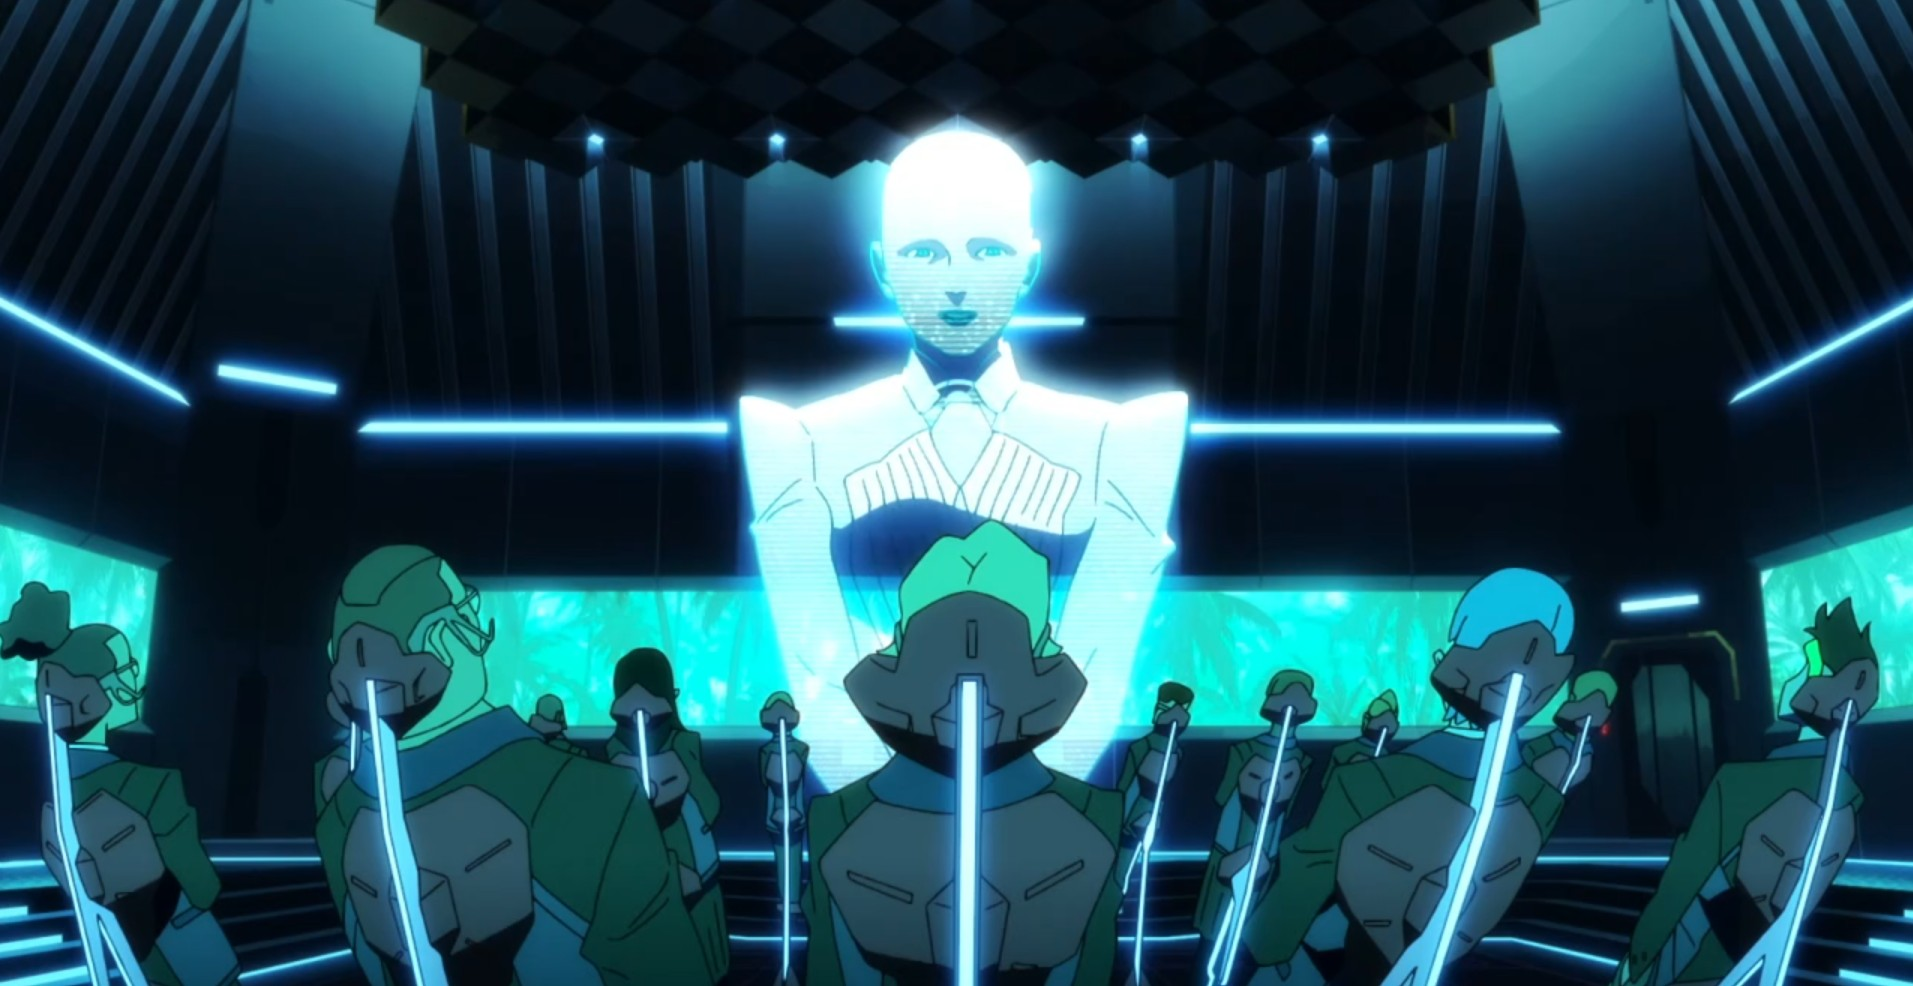
\includegraphics[alt={Figure 1.1},width=0.99\textwidth]{figures/F1-1.jpg}}
    \caption{Virtual Classroom in Cyberpunk: Edgerunners\label{fig:1-1}}
\end{figure}

\textcite{forsler_2024} propose the term “post-digital classroom” to identify the characteristics and trends in education
present in a world beyond the adoption of digital technologies. The purpose of this classroom is not anymore to
introduce new technologies to students, but to implement them as an essential factor of the learning process. The
post-digital classroom is interconnected, social and global. In this scenario, learning goes beyond the physical
classroom because it is based on creating relationships between concepts and developing valuable skills rather than
acquiring knowledge. It is also a classroom where information is detached from the physical learning institute, and
access to facts and sources is, ideally, immediate, ubiquitous and democratic.

\section[Context]{Context}

\section[Research Structure]{Research Structure}
\subsection[Research Questions]{Research Questions}
\subsection[Scope and Limitations]{Scope and Limitations}
\section[Significance and Contributions]{Significance and Contributions}
\section[Document Structure]{Document Structure}